\section{稀疏自编码器}
\subsection{自编码器}
传统反向神经网络缺点:
\begin{itemize}
    \item 梯度越来越稀疏(梯度弥散):从顶层越往下,误差校正信号越来越小;
    \item 容易收敛到局部最小值,尤其是从远离最优区域开始的时候(将参数初始化为随机值会导致这种情况发生);
    \item 只能进行有监督训练,但大部分的数据是没有标签的,而人类的大脑可以从没有标签的数据中学习。
\end{itemize}

\textbf{1986} 年,\textbf{Rumelhart} 提出了自动编码器的概念,并将其用于高维复杂数据的处理,促进了神经网络的发展。
自编码神经网络是一种\textbf{无监督}(自监督)学习算法,它使用了反向传播算法,
并让\textbf{目标值等于输入值},即自编码神经网络尝试学习一个 $h_{W, b}(x) \approx x$ 的函数。

自编码器分类:
\begin{itemize}
    \item 浅层自编码(Autoencoder)
    \item 稀疏自编码(Sparse Autoencoder)
    \item 栈式自编码(Stacked Autoencoder)
    \item 去噪自编码(Denoising Autoencoder)
    \item 变分自编码(Variational Autoencoder)
\end{itemize}

自编码器的共同点:学习一个\textbf{与输入相同的输出},并尽可能的让其具有较强的\textbf{泛化能力}。

自编码器的构成:
\begin{itemize}
    \item 编码器是把高维度数据\textbf{有损的}映射成低维度数据,
    减少数据量,要实现这种映射关系需要学习数据间的相关性,对输入 $x$ 编码,得到新的特征 $y$;
    \item 解码器和编码器完全相反,是把低维度数据映射成高维度数据,\textbf{增加数据量},
    使经过压缩的数据恢复成原来的样子,即利用新的特征 $y$,得到一个重构的数据 $x'$;
    \item 损失函数用来衡量由于压缩而损失掉的信息。编码器和解码器一般都是参数化的方程,
    且关于损失函数\textbf{可导},典型的情况是使用最小均方误差
    \begin{equation}
        \text{MSE} = \dfrac 1n \sum\limits_{i=1}^n (x - x')^2
    \end{equation}
\end{itemize}

\subsection{深度自编码器}
\textbf{2006} 年,\textbf{Hinton} 对原型自动编码器的结构进行了改进,
进而产生了 DAE,先用\textbf{无监督逐层贪心训练算法}完成对隐含层的\textbf{预训练},
然后用\textbf{反向传播}算法对整个神经网络进行系统性参数优化调整,
显著降低了神经网络的训练复杂程度,有效改善了反向传播算法容易陷入局部最小的不良状况。

将三层浅层自编码器扩展成具有多个隐藏层的编码器即为深度自编码器,能更好的学习数据更高维度的特征。

\subsubsection{逐层学习}
在深度自编码器中,对其中的多个隐藏层,我们需要进行逐层自编码学习。
具体地,每一个编码层中都会包含一个解码器,用来输出当前层的解码结果,我们贪心地希望每一层的解码结果都与前一层向其输入的结果尽可能的相似:
\begin{figure}[htbp]
    \centering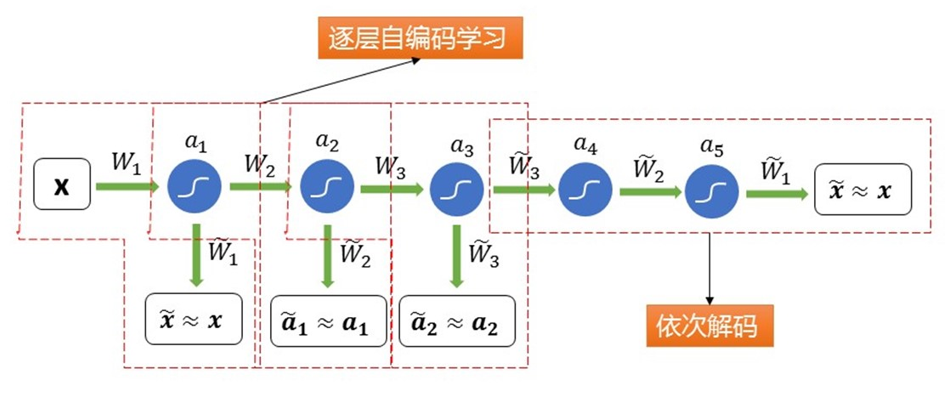
\includegraphics[scale = 0.4]{DAE.png}
\end{figure}

深度自编码器特点:具有强大的\textbf{表达能力}及深度神经网络的\textbf{所有优点}。
它通常能够获取到输入的“层次性分组”或者“部分-整体分解”结构。自编码器倾向于学习得到能更好地\textbf{表示输入数据的特征}。

\subsection{稀疏表示}
我们可以寻找一个系数矩阵 $u$ 和一个字典矩阵 $V$,使得 $V \times u$ 尽可能的还原 $x$,
且 $u$ 尽可能地稀疏,则 $u$ 就是 $x$ 的稀疏表示。我们将一个大矩阵变成两个小矩阵,从而达到压缩的目的。
\begin{figure}[htbp]
    \centering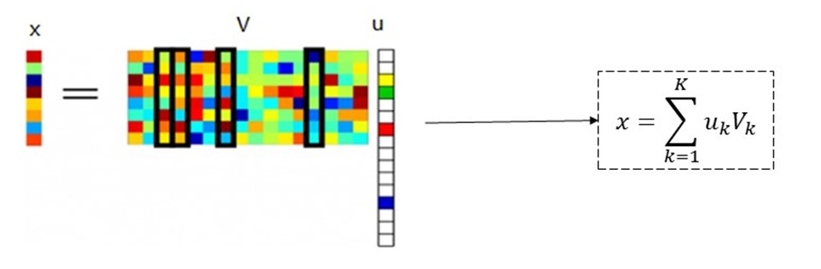
\includegraphics[scale = 0.5]{sparse.png}
\end{figure}

给定数据集 $\left\{\boldsymbol{x}_1, \boldsymbol{x}_2, \dots, \boldsymbol{x}_m\right\}$,字典学习的最简单形式为
\begin{equation}
    J(\mathbf B, \boldsymbol{\alpha}) = \min_{\mathbf B, \boldsymbol{\alpha}_i} \sum_{i=1}^m
    \left\|x_i - \mathbf B \boldsymbol{\alpha}_i\right\|_2^2 
    + \lambda\sum_{i=1}^m\left\|\boldsymbol{\alpha}_i\right\|_1  
\end{equation}

其中 $\mathbf B \in \mathbb{R}^{d \times k}$ 为字典矩阵,$k$ 称为字典的\textbf{词汇量},通常由用户指定。
$\boldsymbol{\alpha}_i \in \mathbb{R}^k$ 则是样本 $\boldsymbol{x}_i \in \mathbb{R}^d$ 的稀疏表示。
显然,上式的第一项是希望 $\boldsymbol{\alpha}_i$ 能较好地重构 $\boldsymbol{x}_i$,
第二项则是希望 $\boldsymbol{\alpha}_i$ 尽量稀疏,可以再加入一项 $+ \beta\sum_r\sum_c \mathbf B_{rc}^2$,表示希望字典中每项也尽可能小。

为了较为简单的最小化上述二元函数,我们通过变量交替优化的策略来进行:
\begin{itemize}
    \item 首先随机初始化字典矩阵 $\mathbf B$;
    \item 然后通过梯度下降,得到 $\mathbf B$ 确定时使得函数 $J(\cdot, \cdot)$ 取得最小值时的 $\boldsymbol{\alpha}$;
    \item 再通过梯度下降,得到 $\boldsymbol{\alpha}$ 确定时使得函数 $J(\cdot, \cdot)$ 取得最小值时的 $\mathbf B$;
    \item 不断重复上述两步,直至结果确定。
\end{itemize}

\subsection{稀疏自编码}

一个神经网络中,使得神经元在大部分的时间内都是被\textbf{抑制}的限制称为\textbf{稀疏性限制}。

考虑一个最简单的自编码器,其神经网络只有三层,那么 $a_j^{(2)}$ 表示隐藏层中的隐藏神经元 $j$ 的激活值,
但这种表示方法无法表示是哪一个输入 $x$ 带来的激活值,所以我们改用 $a_j^{(2)}(x)$ 表示在给定输入为 $x$ 的情况下,
隐藏层中的隐藏神经元 $j$ 的激活值。

令
\begin{equation}
    \hat{\rho}_j = \dfrac 1m \sum_{i=1}^m{a_j^{(2)}(x^{(i)})}
\end{equation}

表示隐藏神经元 $j$ 在 $m$ 个输入样本上的平均激活度。

再近似的加入一条限制:$\hat{\rho}_j = \rho$,其中 $\rho$ 被称为稀疏性参数。
为了满足这一限制,将会在优化目标函数中加入一个惩罚因子,
这将惩罚那些 $\hat{\rho}_j$ 和 $\rho$ 有显著不同的情况,从而使得隐藏神经元的平均活跃度保持在较小范围内。

\subsubsection{KL 散度}
定义两分布 $P$,$Q$ 之间的相对熵(KL 散度)为
\begin{equation}
    D(P\|Q) = \sum_xE\left[\ln p(x) - \ln q(x)\right] = \sum_xp(x) \ln \dfrac{p(x)}{q(x)}
\end{equation}

其中 $p(x)$,$q(x)$ 为两分布的概率密度函数。
相对熵可以解释为“通过 $q$ 的编码去编码 $p$后,信息丢失数的期望”,可以用相对熵来表示两个分布之间的差异。

把隐层的每个神经元的激活和未激活态看做服从\textbf{二项分布},
则 KL 散度可以表示为一个以 $\rho$ 为均值和一个以 $\hat{\rho}_j$ 为均值的两个二项分布之间的相对熵:
\begin{equation}
    \operatorname{KL}(\rho \| \hat{\rho}_j) = 
    \rho\ln\dfrac{\rho}{\hat{\rho}_j} + (1 - \rho) \ln \dfrac{1 - \rho}{1 - \hat{\rho}_j}
\end{equation}

KL 散度的三个特点:
\begin{itemize}
    \item $\operatorname{KL}(\rho \| \hat{\rho}_j) \geq 0$,当且仅当 $\rho = \hat{\rho}_j$ 时取等号;
    \item 非对称性:$\operatorname{KL}(\rho\|\hat{\rho}_j) \neq \operatorname{KL}(\hat{\rho}_j\|\rho)$;
    \item 当 $\hat\rho_j \to 0 \text{ or } 1$ 时,$\operatorname{KL}(\rho \| \hat\rho_j) \to +\infty$。
\end{itemize}

现在,代价函数可以表示为
\begin{equation}
    J_{\text{sparse}}(\mathbf B, \boldsymbol{\alpha}) 
    = J(\mathbf B, \boldsymbol{\alpha}) + \beta\sum_{j=1}^{s_2}\operatorname{KL}(\rho\|\hat{\rho}_j)
\end{equation}

注意到
\begin{equation}
    \dfrac{\partial \operatorname{KL}(\rho \| \hat{\rho}_j)}{\partial \hat{\rho}_j} 
    = -\dfrac{\rho}{\hat{\rho}_j} + \dfrac{1 - \rho}{1 - \hat{\rho}_j}
\end{equation}

于是在神经网络的反向传播中,当前层误差 $\delta^{(l)}$ 更新为
\begin{equation}
    \delta^{(l)} = \left((\omega^{(l+1)})^\mathrm{T}\delta^{(l+1)} 
    + \beta\left(-\dfrac{\rho}{\hat{\rho}_j} + \dfrac{1 - \rho}{1 - \hat{\rho}_j}\right)\right) 
    \odot g'\left(z^{(l)}\right)
\end{equation}

即可,其中 $l = n_l - 1, n_l - 2, \dots, 2$。
注意,在进行稀疏自编码器的训练过程中,必须要先进行一次前向传播以得到所有神经元的平均激活度 $\hat{\rho}$。